% Markdown 方案的续写部分。
% example.tex 已包含总体技术路线至发作状态识别模型设计，此处从第五部分开始，避免重复。

\clearpage
\section{发作起始点定位方法}

\subsection{操作性定义与标注对齐}

医学判读中，“最早可疑电图变化”“最早明确电图发作变化”“首批通道持续募集”和“首次临床症状”可能对应不同时间点。竞赛训练与评价首先服从官方标注定义；若官方只给出 onset 数值而未说明标注准则，本方案将其作为数据集操作性边界，不擅自解释为真实 EZ 的启动时刻，并在答疑阶段请求确认其对应的电图或临床标准。

\begin{figure}[htbp]
\centering
\begin{tikzpicture}[
    node distance=5mm and 3mm,
    box/.style={draw, rounded corners=1pt, align=center, font=\zihao{-5}, text width=2.55cm, minimum height=1.05cm, inner sep=3pt},
    arrow/.style={-{Latex[length=1.5mm]}, line width=0.45pt}
]
    \node[box] (ueo) {最早可疑变化\\UEO};
    \node[box, right=of ueo] (eec) {最早明确电图变化\\EEC／候选 onset};
    \node[box, right=of eec] (recruit) {首批通道持续募集\\起始候选与早期传播};
    \node[box, right=of recruit] (clinical) {首次临床症状\\临床 onset};
    \node[box, right=of clinical] (late) {晚期传播\\广泛同步};
    \draw[arrow] (ueo) -- (eec);
    \draw[arrow] (eec) -- (recruit);
    \draw[arrow] (recruit) -- (clinical);
    \draw[arrow] (clinical) -- (late);
\end{tikzpicture}
\caption{不同 onset 相关时间点的操作性区分；实际监督目标以官方标注为准}
\label{fig:onset-timeline}
\end{figure}

训练前须形成 onset 标注审计表，记录标注来源、时间分辨率、取整方式、是否允许多起始事件、片段左删失与右删失规则以及多专家差异。模型输出精度不得高于数据和帧率所支持的实际时间分辨率。

\subsection{两阶段去循环推理}

动态基线和募集证据依赖 onset 邻域，而 onset 又可能受动态图影响。为消除循环依赖，第一阶段只使用默认时域--时频链路得到粗状态序列和粗 onset；第二阶段仅在粗 onset 前存在足够质量合格基线时，计算相对基线动态图与募集矩阵，再对边界进行精修。左删失或基线不足时跳过片段内差分图，不能用真实测试标注构建基线。

\begin{figure}[htbp]
    \centering
    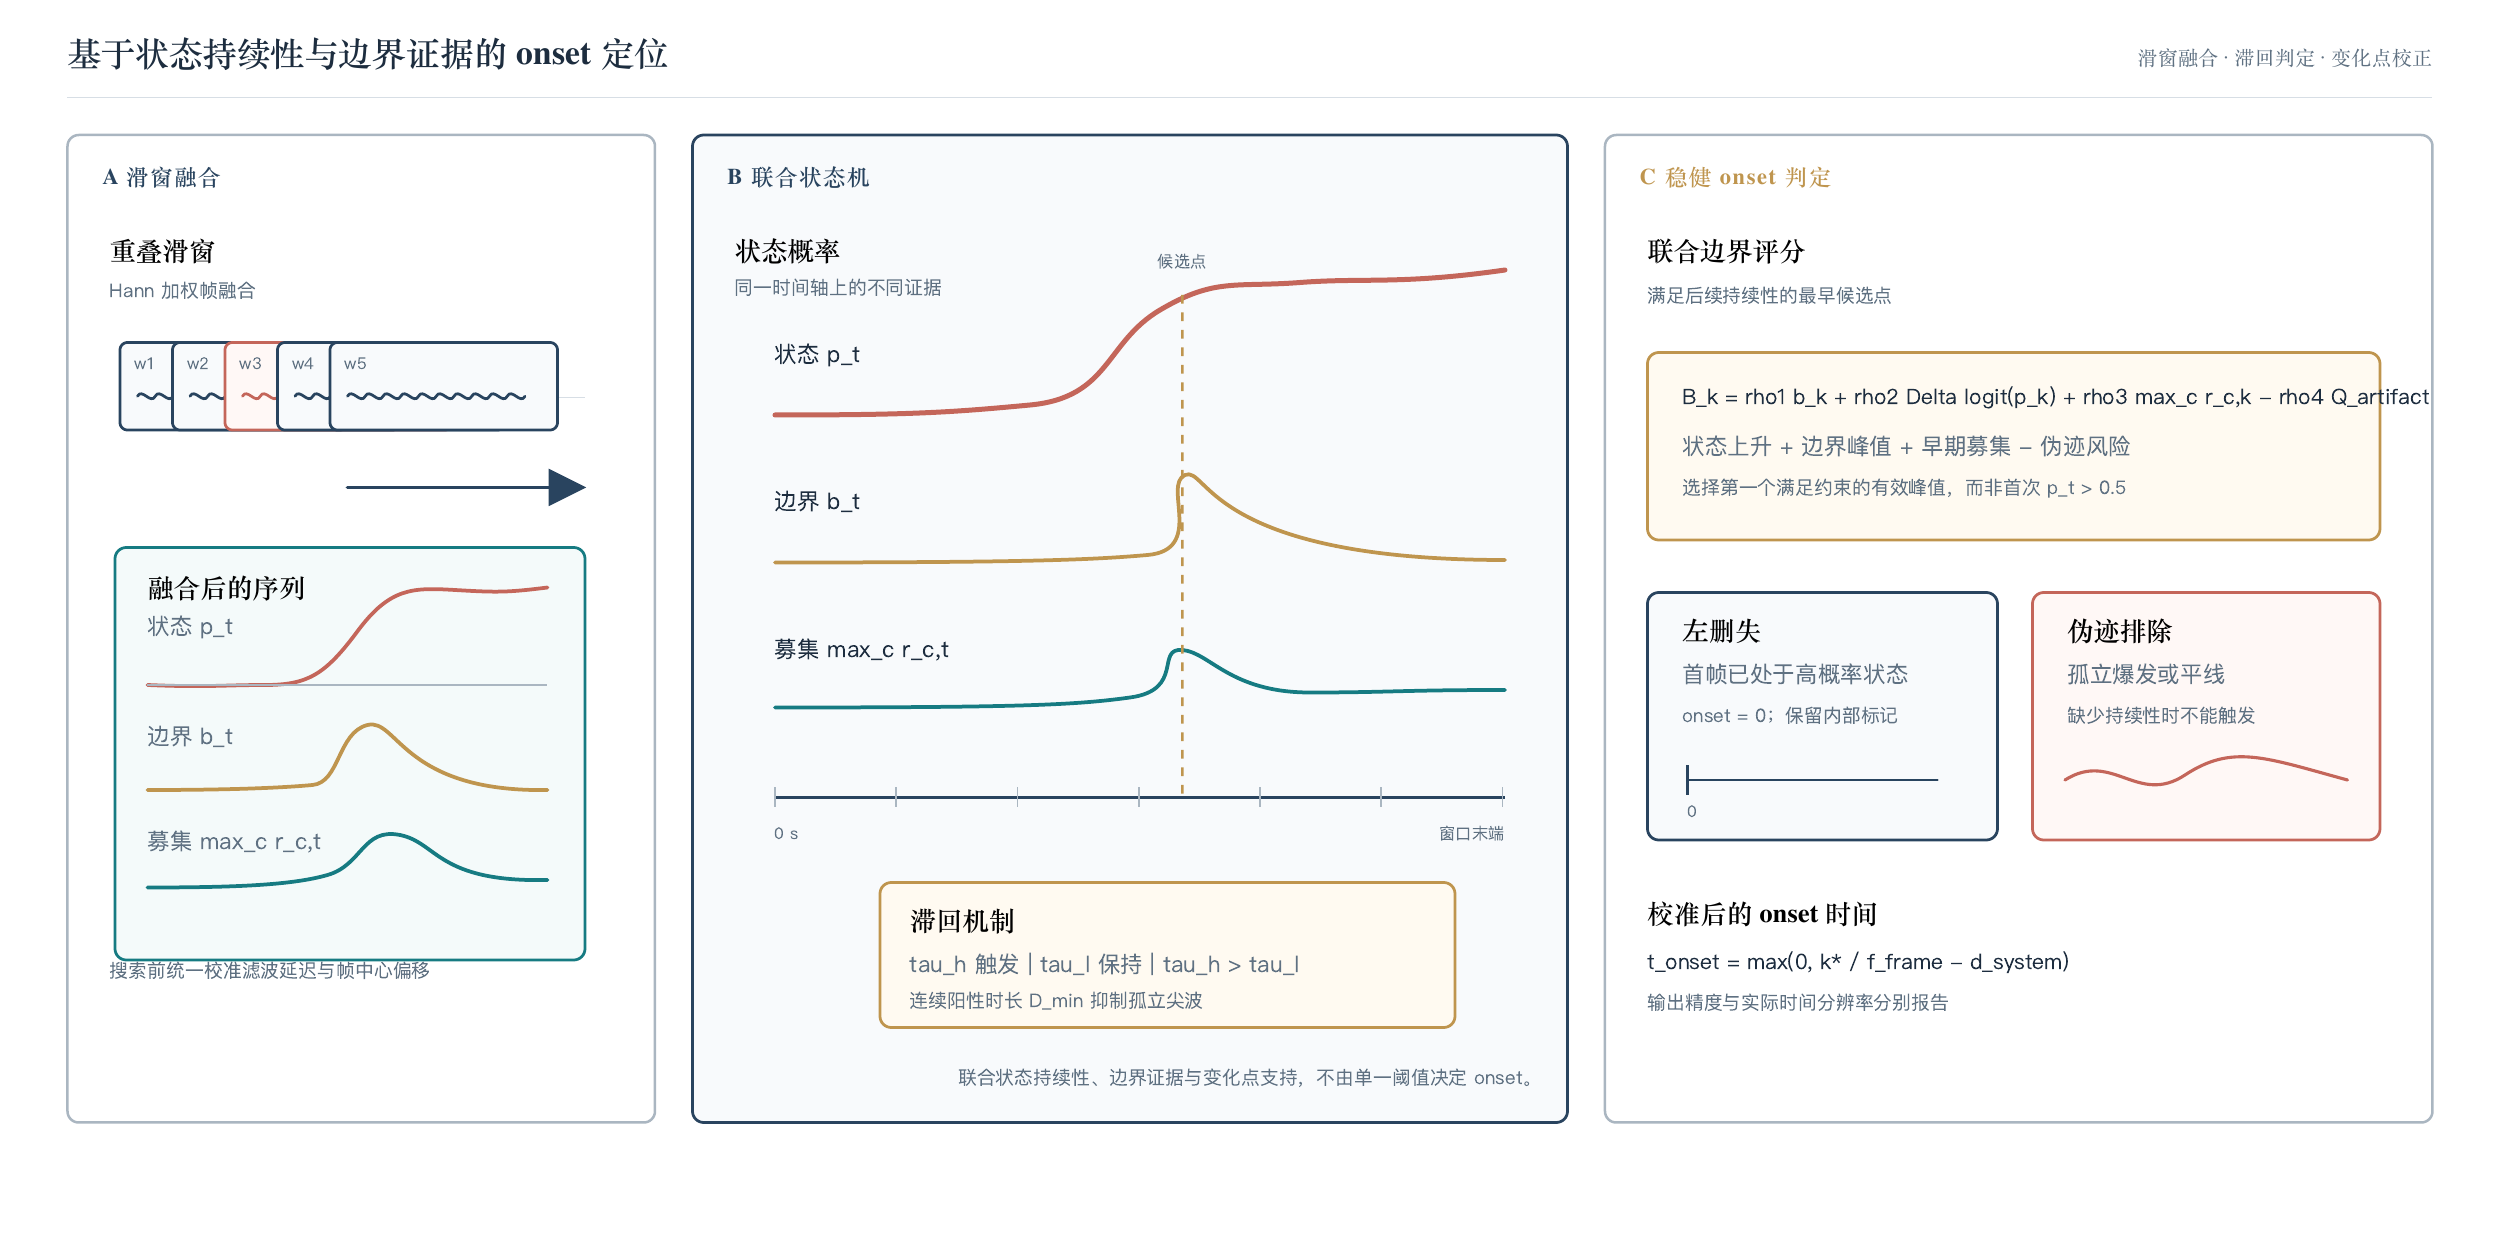
\includegraphics[width=\linewidth]{tmp/pdfs/seeg_figures_zh_final/onset-1.png}
    \caption{状态持续性、边界与募集证据联合的 onset 判定；V2 在其前增加粗定位阶段以构建无泄漏基线}
    \label{fig:onset-localization}
\end{figure}

\subsection{状态与边界概率重建}

对长片段执行重叠窗口推理后，同一时间帧可能获得多个状态概率和边界概率。两类序列分别采用窗口中心加权方式融合：

$$
\bar p_k=
\frac{\sum_w q_{w,k}p_{w,k}}
{\sum_w q_{w,k}+\varepsilon},
$$

其中 $q_{w,k}$ 为三角形或 Hann 权重，使窗口边缘的低可靠预测贡献较小；边界概率采用相同方法得到 $\bar b_k$。滤波群延迟、模型感受野中心偏移及重采样时间映射在此阶段统一补偿。

\subsection{概率平滑与阈值滞回}

首先对 $\bar p_k$ 进行 0.25～0.75 s 中值滤波，去除孤立尖峰；随后使用指数移动平均或一维高斯滤波。平滑尺度通过患者级验证确定，避免过强平滑造成 onset 系统性延后。

状态机采用双阈值滞回机制。高阈值 $\tau_h$ 用于触发候选发作，低阈值 $\tau_l$ 用于维持发作状态，且 $\tau_h>\tau_l$。候选 onset 需满足：状态概率越过高阈值；边界概率在前后容忍区间内存在局部峰值；后续至少 $D_{\min}$ 秒内大部分帧高于低阈值；候选区间平均概率和上升斜率达到最低要求；低质量伪迹帧不能独立触发发作。

连续阳性约束用于抑制短暂尖波、电极爆裂和单帧模型波动。$\tau_h$、$\tau_l$ 和 $D_{\min}$ 均由训练折内部验证确定。

\subsection{联合边界判定与变化点校正}

状态概率确定发作持续区间，边界概率提供状态转变的直接定位证据。候选区间内首先计算联合边界分数：

$$
B_k=\rho_1\bar b_k
+\rho_2\Delta\mathrm{logit}(\bar p_k)
+\rho_3\max_c r_{c,k}
-\rho_4Q_k^{\mathrm{artifact}},
$$

其中 $r_{c,k}$ 为通道募集强度，$Q_k^{\mathrm{artifact}}$ 为伪迹风险。选择满足后续状态持续性约束的最早显著峰值作为初始 onset。变化点检测不再承担主要定位任务，而作为边界头的独立校正证据。在初始 onset 前的限定区间内构造：

$$
R_k=
w_p\Delta\mathrm{logit}(\bar p_k)
+w_e\Delta E_k
+w_s\Delta S_k,
$$

其中，$\Delta E_k$ 表示判别频带能量相对基线的变化，$\Delta S_k$ 表示动态功能图相对基线的变化。工程实现固定使用经验证表现最优的一种变化点算法；CUSUM 和 PELT 仅作为消融候选，不在正式链路中并行运行。最终 onset 由状态持续区间、边界峰值和变化点证据联合确定，不采用“首次超过 0.5”作为唯一规则。

时间输出为：

$$
t_{\mathrm{onset}}=
\max\left(0,\frac{k^*}{f_{\mathrm{frame}}}-d_{\mathrm{system}}\right),
$$

其中 $d_{\mathrm{system}}$ 为滤波和模型引入的标定延迟。输出数值精度与模型实际时间分辨率需区分；例如帧间隔为 0.125 s 时，即使结果格式保留三位小数，也不能据此声称达到毫秒级定位精度。

\subsection{异常片段处理与定位置信度}

若最终标签为 0，则 onset 输出空值、\texttt{null} 或官方规定的占位符。若标签为 1 且首帧已持续处于高概率状态，说明发作可能在片段开始前发生，此时 onset 置为 0，并在内部记录 \texttt{left\_censored=true}。若高概率区仅位于补齐区域，则不得将其作为 onset。

定位置信度综合考虑阈值裕量、持续时间、概率上升斜率、变化点显著性及重叠窗口一致性：

$$
Q_{\mathrm{onset}}=
\eta_1Q_{\mathrm{margin}}
+\eta_2Q_{\mathrm{duration}}
+\eta_3Q_{\mathrm{change}}
+\eta_4Q_{\mathrm{agreement}}.
$$

若提交格式不允许输出置信度，该值仍保留在内部日志中，用于错误分析和临床辅助场景下的低置信提示。

\clearpage
\section{关键通道识别与候选起始网络估计}

比赛要求按照模型贡献度输出当前片段最重要的 10 个通道。模型贡献与临床起始先后并不等价：晚期传播通道可能强烈影响分类，最早募集通道也可能因低幅而具有较小的片段分类贡献。因此 V2 明确分离“比赛解释分数”和“临床早期分数”，避免使用一个含义混合的 Top-10 同时声称完成两类目标。

\subsection{比赛解释分数与临床早期分数}

比赛解释分数首先回答“模型为什么作出当前判断”：

$$
S_c^{\mathrm{comp}}=
a_1M_c^{\mathrm{model}}
a_2O_c^{\mathrm{proxy}}
a_3U_c^{\mathrm{stable}}
-a_4Q_c^{\mathrm{artifact}},
$$

其中 $M_c^{\mathrm{model}}$ 为一次前向得到的通道贡献，$O_c^{\mathrm{proxy}}$ 为经离线遮挡蒸馏得到的快速近似，$U_c^{\mathrm{stable}}$ 为扰动稳定性，$Q_c^{\mathrm{artifact}}$ 为质量惩罚。该分数通过充分性、必要性和随机等规模通道遮挡验证，作为官方 Top-10 的默认依据。

临床早期分数回答“哪些接点更早表现出持续募集和领先关系”，仅用于候选起始接点及传播分层。

\subsection{onset 感知的证据窗口}

阳性样本的主要评分区间限定为：

$$
\mathcal{W}_{\mathrm{early}}=
[t_{\mathrm{onset}}-\delta_1,
t_{\mathrm{onset}}+\delta_2],
$$

其中 $\delta_1$ 用于覆盖边界标注误差及 onset 前最早变化，$\delta_2$ 限制晚期传播影响，初值分别可设为 1～2 s 和 3～5 s。若片段左删失或 onset 置信度较低，则扩大时间窗并降低早期性项权重。晚期区间只用于判断传播层级，不参与起始候选的主要排序。

\subsection{临床早期通道评分}

临床辅助链路采用一次模型前向即可获得的证据：

\[
\begin{aligned}
S_c^{\mathrm{clinical}}={}&
w_1E_c^{\mathrm{early}}+w_2L_c^{\mathrm{latency}}
+w_3D_c^{\mathrm{evolution}}+w_4P_c^{\mathrm{outflow}}\\
&+w_5R_c^{\mathrm{repeat}}+w_6M_c^{\mathrm{model}}
-w_7Q_c^{\mathrm{artifact}}.
\end{aligned}
\]

其中：

\begin{itemize}[leftmargin=2em,itemsep=0.2em]
    \item $E_c^{\mathrm{early}}$ 为 onset 邻域内的募集强度及相对基线异常幅度；
    \item $L_c^{\mathrm{latency}}$ 为通道首次持续募集相对全局 onset 的潜伏期，激活越早得分越高；
    \item $D_c^{\mathrm{evolution}}$ 描述节律持续性、频率迁移、振幅演化和线长变化，用于区别发作演化与孤立棘波；
    \item $P_c^{\mathrm{outflow}}$ 为动态有向功能图中的净外流及其相对基线增量，用于识别传播上游通道；
    \item $R_c^{\mathrm{repeat}}$ 为同一患者多次发作间的排名一致性；单次发作或未知患者时该项置为中性，不以缺失信息惩罚；
    \item $M_c^{\mathrm{model}}$ 为募集头置信度和轻量注意力贡献；
    \item $Q_c^{\mathrm{artifact}}$ 为坏道、饱和、工频和宽带伪迹风险。
\end{itemize}

各分量采用样本内百分位秩归一化，权重由患者级验证集学习或网格搜索确定，并设置非负与和为 1 的约束。任何单一能量指标均不得主导总分。默认提交使用 $S_c^{\mathrm{comp}}$ 排序；只有官方答疑或评价标准明确要求起始相关通道时，才在训练前固定融合系数，将 $S_c^{\mathrm{clinical}}$ 纳入提交分数。临床报告始终单独展示两套分数及其含义。评分后先剔除无效通道，再输出官方定义的通道 ID。

对阴性样本，比赛若仍要求 Top-10，则输出“对发作间期判定最具信息量且质量可靠的通道”，评分由状态头贡献、背景稳定性和低伪迹风险构成；该排序不使用 onset 潜伏期，也不解释为起始区候选。

\subsection{起始与传播分层}

根据募集时间 $t_c^{\mathrm{recruit}}$ 和有向领先关系，将阳性通道在内部划分为：onset 容忍区间内首先持续激活且具有较高统计外流的起始候选；随后短延迟激活的早期传播通道；以及在广泛同步阶段才激活的晚期传播通道。官方 Top-10 仍由比赛解释分数产生；临床复核报告另行展示传播分层及每个通道的募集潜伏期，避免把模型贡献、晚期传播和起始候选混为一谈。

\subsection{离线归因验证}

Integrated Gradients、SmoothGrad 和通道遮挡不进入每个测试样本的正式低时延链路，而用于模型验证和疑难病例复核。遮挡贡献定义为：

$$
O_c=z(X)-z(X_{\setminus c}).
$$

在验证集上检查快速评分 Top-$k$ 通道被遮挡后，片段 logit、边界概率和募集一致性是否显著下降，并与随机通道遮挡比较；积分梯度用于核验模型是否依赖 onset 早期而非片段末端。若快速评分与离线归因长期不一致，则调整募集头监督和评分权重，而不是在正式推理中堆叠全部归因方法。

\subsection{稳定性与临床可读性}

在轻微噪声、时间偏移和通道缺失扰动下重复评估，分别报告比赛 Top-10 的 Jaccard、Spearman/Kendall 相关，以及临床早期排序的 onset 潜伏期方差。同一患者存在多次发作时，另计算临床早期排序的跨发作重复性；两套排序不得在报告中合并为一个未经定义的指标。

Top-10 只表示当前植入覆盖范围内、与本次记录状态转变相关的重要通道。有效通道少于 10 个时不伪造通道，按官方规则补空值或无效占位符。算法结果不自动定义 SOZ、EZ 或手术切除范围。

\subsection{空间约束与脑区级聚合（条件模块）}

在具备可靠接点坐标时，将欧氏距离、同一电极杆关系和可选脑区邻接作为静态空间先验，与时变功能图共同约束传播路径。空间先验不覆盖信号证据：较远接点之间若存在稳定的有向传播关系仍可保留连接，近邻接点也不能仅因距离接近而被判为共同起始。

在具备 CT--MRI 配准和个体脑区映射时，将接点分数聚合为脑区级候选分数：

$$
S_r^{\mathrm{ROI}}=
\frac{\sum_c\omega_{c,r}\,q_c^{\mathrm{coord}}\,\sigma(S_c^{\mathrm{clinical}})}
{\sum_c\omega_{c,r}\,q_c^{\mathrm{coord}}+\varepsilon},
$$

其中 $\omega_{c,r}$ 为接点 $c$ 属于脑区 $r$ 的软映射权重，$q_c^{\mathrm{coord}}$ 为坐标和配准质量，$S_c^{\mathrm{clinical}}$ 为接点级临床早期分数。若没有人工 SOZ 脑区标签，$S_r^{\mathrm{ROI}}$ 只能称为候选分数；只有经患者级校准和独立验证后，才可表述为概率。脑区聚合用于临床复核报告，不改变比赛必须输出的原始 Top-10 通道 ID。

根据可用数据，定位能力按下表分级启用：

\begin{table}[htbp]
    \centering
    \zihao{5}\small
    \caption{定位能力与数据条件}
    \label{tab:space-levels}
    \renewcommand{\arraystretch}{1.25}
    \setlength{\tabcolsep}{3pt}
    \begin{tabularx}{\linewidth}{@{}p{0.23\linewidth}p{0.35\linewidth}X@{}}
        \toprule
        \textbf{可用数据} & \textbf{可实现输出} & \textbf{明确限制} \\
        \midrule
        SEEG 波形和通道 ID & 候选起始通道、募集顺序、早期传播关系 & 不能称为严格脑源成像，不能定位未覆盖脑区 \\
        接点三维坐标 & 空间约束动态图、接点级三维传播路径 & 只描述已植入接点之间的空间关系 \\
        术前 MRI、术后 CT 和解剖分区 & 接点—脑区映射、脑区级候选分数及空间展示 & 结果受配准、分区和植入覆盖范围限制 \\
        专家 SOZ 标注 & 接点或脑区级监督与概率校准 & 标签存在阅图者差异，需多专家或裁决标准 \\
        实际处理区域及术后结局 & 定位结果与临床疗效的回顾性关联验证 & 处理区域不等同于真实 EZ，不能据此单独证明因果性 \\
        MRI、DWI 和结构连接组 & 患者特异性结构先验或研究性生物物理模型 & 数字孪生、虚拟切除不进入本竞赛主流程 \\
        \bottomrule
    \end{tabularx}
\end{table}

\subsection{定位不确定性与弃权机制}

定位置信度综合 onset 不确定性、通道排名扰动稳定性、跨发作一致性、坐标配准误差和植入覆盖充分性：

$$
Q_{\mathrm{loc}}=
f(Q_{\mathrm{onset}},Q_{\mathrm{rank}},Q_{\mathrm{repeat}},
Q_{\mathrm{coord}},Q_{\mathrm{coverage}}).
$$

其中覆盖充分性只评价“现有接点是否形成稳定、可解释的早期上游模式”，不能证明未覆盖脑区不存在真实起始源。出现接点坐标缺失、配准误差超限、多个候选区域分数接近、不同发作定位不一致、严重伪迹或无稳定上游接点时，系统停止输出脑区级肯定结论，并提示“定位证据不足，需复核植入覆盖与原始波形”。比赛若强制输出 Top-10，仍按官方格式给出通道排序，但内部低置信标记必须保留，且不得将强制输出解释为可靠定位。

$Q_{\mathrm{loc}}$ 的各分量统一归一化至 $[0,1]$，函数 $f$ 采用具有单调约束的逻辑模型或保序校准，并只在患者级验证集上拟合。没有可靠空间参考标准时，$Q_{\mathrm{loc}}$ 仅称为定位质量指数，不表述为“定位正确概率”。

\clearpage
\section{推理与部署方案}

\subsection{完整推理流水线}

正式推理包含以下环节：

\begin{enumerate}[leftmargin=2.6em,itemsep=0.2em]
    \item 读取样本及元信息，核验采样率、通道 ID、张量方向、数值类型和有效长度。
    \item 执行重采样、滤波、质量检测、参考重构和稳健标准化。
    \item 生成重叠滑窗、通道掩码及帧有效掩码。
    \item 执行第一阶段默认链路，获得片段概率、帧级状态概率、边界概率和粗 onset。
    \item 若粗 onset 前存在足够质量合格基线，则执行第二阶段动态图与募集分支并精修 onset；否则跳过片段内差分图。
    \item 融合窗口结果并执行概率校准，得到最终发作概率和二分类标签；仅对阳性样本输出 onset。
    \item 使用比赛解释分数 $S_c^{\mathrm{comp}}$ 生成官方 Top-10；临床早期分数仅进入内部复核报告。
    \item 若坐标和影像映射可用且通过质控，生成接点级三维传播路径、脑区候选分数和定位置信度；否则跳过该条件模块。
    \item 按官方模板完成字段、数值精度、通道顺序和缺失值格式化，并运行提交校验程序。
\end{enumerate}

建议的中间结果结构如下：

\begin{verbatim}
{
  "sample_id": "sample_xxx",
  "label": 1,
  "probability": 0.873421,
  "top10_channels": [
    "A3", "A4", "B2", "A2", "C7",
    "B3", "D1", "C6", "A5", "D2"
  ],
  "onset_time": 12.375
}
\end{verbatim}

实际字段名称、分隔符和空值表达以官方模板为准。概率先校准、后格式化；标签使用未舍入概率判定，避免临界概率因六位小数截断而与标签不一致。

\subsection{快速推理与深度解释分层}

比赛正式提交和准实时筛查采用快速链路。无动态基线条件时只需一次默认链路前向；启用动态图精修时执行两阶段前向，并单独计入端到端时延。官方 Top-10 使用已蒸馏的快速贡献头，不依赖在线反向传播或逐通道重复前向。

离线验证和临床疑难片段复核可启用深度解释链路，执行 Integrated Gradients、SmoothGrad、通道遮挡和多扰动稳定性分析。两套链路的作用不同：快速链路满足时延约束，深度解释链路验证快速通道排序是否可信，不将后者的计算成本计入基础模型前向耗时，但在完整临床系统评估中单独报告。

\subsection{GPU 部署}

GPU 模式采用 FP16 或 BF16 混合精度，窗口按样本动态批处理。预处理尽量采用向量化 CPU 实现并使用固定内存缓存，模型输入通过 pinned memory 异步传输。深度解释模式需要遮挡时，将候选组成扩展 batch 一次前向，但该步骤不进入正式快速链路。

\subsection{CPU 部署}

CPU 模式优先使用深度可分离卷积、稀疏 Top-$k$ 图和 TCN，限制全局自注意力规模。通过 ONNX Runtime 或 OpenVINO 执行算子融合、线程绑定和 INT8 推理。STFT、滤波和窗口生成使用连续内存布局，避免在通道维反复复制。

\subsection{时延与内存控制}

推理耗时分解为数据读取、预处理、模型前向、onset 后处理、通道解释和结果格式化六部分。分别报告冷启动和稳态耗时，并给出 P50、P95，而不只报告单次最优值。

内存侧采用流式读取、滑窗环形缓存和按块推理，不将超长记录的所有窗口一次性展开。重叠窗口共享滤波结果、STFT 帧和局部编码特征。在未明确比赛硬件前，不预设绝对毫秒级目标；模型定型后应在目标环境进行批量大小、线程数和精度模式的联合寻优。

\subsection{异常输入处理}

对空文件、NaN/Inf、采样率缺失、通道重复、通道数不足、片段过短和极端幅值设置确定性处理规则。无法恢复的通道置无效掩码；片段过短时反射补齐，并禁止在补齐区域输出 onset；全部通道失效时输出低置信默认结果和错误码，避免程序崩溃或生成非数值概率。

\clearpage
\section{模型轻量化与算力优化}

轻量化不与核心模型创新并列。正式优化主线限定为“教师—学生蒸馏、混合精度或 INT8、滑窗缓存复用”三项；结构化剪枝、低秩分解仅在目标硬件基准显示存在实际瓶颈时启用，避免形成与收益无关的技术堆叠。

首先训练完整教师模型，再训练轻量学生模型。学生模型保留共享时域编码、频带增强和帧级输出，但减少通道图层数、隐藏维度和时序块数量。蒸馏目标包括片段 logit、帧级概率、中间时序特征及通道排名：

$$
\mathcal{L}_{\mathrm{KD}}=
\alpha\mathcal{L}_{\mathrm{logit}}
+\beta\mathcal{L}_{\mathrm{frame}}
+\chi\mathcal{L}_{\mathrm{feature}}
+\delta\mathcal{L}_{\mathrm{rank}}.
$$

通道排名蒸馏用于限制模型压缩后的解释漂移。若蒸馏后仍不能满足算力预算，再采用结构化剪枝，剪枝对象限定为卷积输出通道、注意力头和图层宽度，并在每轮剪枝后微调。非结构化稀疏若不能在目标硬件获得实际加速，不纳入正式方案。

CPU 部署优先量化卷积和线性层至 INT8；归一化、Softmax、概率输出和 onset 后处理保留 FP16 或 FP32。若静态量化导致低幅发作特征损失，则采用量化感知训练，或只量化时域编码器和分类头。

动态图仅保留 Top-$k$ 边，连接估计使用降采样特征。大尺寸线性映射只有在 profiling 证明其为主要耗时来源时才进行低秩分解。通道数较多时，可先以质量评分屏蔽坏道，但不为减少计算而任意删除低幅通道，以免漏掉局灶性起始活动。

连续滑窗共享滤波数据、STFT 帧和部分卷积状态。以 4 s 窗口、0.5 s 步长为例，直接重复编码会产生显著冗余；采用流式编码后，仅需计算新增 0.5 s 数据对应的局部特征。

\begin{table}[htbp]
    \centering
    \zihao{5}\small
    \caption{不同部署场景的模型格式与优化方式}
    \label{tab:deployment}
    \renewcommand{\arraystretch}{1.25}
    \setlength{\tabcolsep}{3pt}
    \begin{tabularx}{\linewidth}{@{}p{0.22\linewidth}p{0.28\linewidth}X@{}}
        \toprule
        \textbf{部署场景} & \textbf{推荐格式} & \textbf{主要优化方式} \\
        \midrule
        NVIDIA GPU & ONNX + TensorRT & FP16、静态形状桶、算子融合、快速通道评分 \\
        x86 CPU & ONNX Runtime / OpenVINO & INT8、线程绑定、图优化、内存复用 \\
        PyTorch 环境 & TorchScript & 脚本化预处理、固定推理图、混合精度 \\
        研究复现 & PyTorch + ONNX 双版本 & 保留训练模型并验证导出误差 \\
        \bottomrule
    \end{tabularx}
\end{table}

轻量化模型须同时满足分类概率误差、onset 偏移和 Top-10 排名稳定性约束。建议将相对教师模型 AUC 下降不超过 0.5～1.0 个百分点、onset MAE 增幅不超过 10\%、Top-10 Jaccard 降幅不超过预设阈值作为初始准入条件，再比较参数量、FLOPs 和端到端时延收益。

\clearpage
\section{训练验证与消融实验设计}

\subsection{实验层级}

实验采用“审计基线—强基线—候选主模型—部署模型”四级体系，不预设复杂模型必然最优。

\begin{table}[htbp]
    \centering
    \zihao{5}\small
    \caption{训练验证的实验层级}
    \label{tab:experiment-levels}
    \renewcommand{\arraystretch}{1.25}
    \setlength{\tabcolsep}{3pt}
    \begin{tabularx}{\linewidth}{@{}p{0.17\linewidth}p{0.36\linewidth}X@{}}
        \toprule
        \textbf{层级} & \textbf{模型与输入} & \textbf{主要作用} \\
        \midrule
        审计基线 & 线长、Hjorth 参数、分频带功率、谱熵、峰度、通道相关统计与 LightGBM & 检查数据基本可分性、识别元数据或幅值泄漏、建立可解释性能下界 \\
        强基线 & 多尺度共享 TCN、掩码通道池化与状态输出头 & 检验不使用动态图时的稳健上限，作为复杂结构的主要对照 \\
        候选主模型 & QST-DPGNet：时域—时频编码、动态双图、状态—边界—募集联合头 & 验证状态转变、传播建模和通道忠实性假设 \\
        部署模型 & 经蒸馏及目标硬件优化的学生模型 & 在分类、onset 和排序退化受控的条件下降低时延和内存 \\
        \bottomrule
    \end{tabularx}
\end{table}

手工特征基线和强基线使用与主模型完全相同的患者级数据划分、窗口定义和概率校准。只有候选主模型在患者级重复验证中稳定超过强基线，改善幅度大于折间波动，且 onset、校准、Top-10 忠实性及推理预算均满足预设门槛时，才进入最终方案；否则采用强基线或删除无稳定增益的模块。

所有模型使用相同的患者级训练、验证和测试划分。数据规模允许时采用五折 GroupKFold；患者数量较少时采用留一患者或重复分组交叉验证。模型选择、阈值优化和概率校准只在训练折内部完成。若数据包含采集时间或中心信息，在患者隔离基础上增加时间外和中心外验证；空间定位结果不得只在参与建模的同中心植入模板上评价。

模型选择采用预先备案的层级规则：先满足 Recall 下限和官方格式校验，再按官方主指标选择；官方主指标尚未公布时，以患者宏 PR-AUC 为首要内部指标。候选差异不超过重复折波动时，依次选择 onset MAE 更低、校准更好且 P95 时延更短的模型，不使用未定义的多指标线性和分数掩盖任务间权衡。

\subsection{评估指标}

分类指标包括 ROC-AUC、PR-AUC、F1、Recall、Specificity、Balanced Accuracy 和期望校准误差 ECE。类别高度不平衡时，PR-AUC 和患者宏平均 F1 作为重点指标。若提供连续记录，进一步报告事件级敏感性、每小时或每天假阳性事件数及检测延迟；若只有独立片段，则明确说明无法从该数据可靠估计连续监测假警报率。

除总体结果外，报告患者宏平均、患者间标准差和 bootstrap 置信区间，并按发作类型、脑区、MRI 阴性或阳性、植入通道数量和信号质量分层。分层样本不足时只进行描述性分析，不据小样本作确定性结论。

onset 定位报告 MAE、中位绝对误差、误差四分位数、平均有符号误差，以及落在 $\pm0.5$ s、$\pm1$ s 和 $\pm3$ s 范围内的比例。平均有符号误差用于识别系统性提前或延迟。左删失、缓慢起始、多起始事件和专家分歧较大的样本分别统计；具备多专家标注时，将模型误差与专家间差异同时报告。

通道评价分为两组。比赛解释分数报告仅保留 Top-10 后的性能保持率、遮挡 Top-10 后的 logit 下降、相对随机遮挡增益、Jaccard 与排名相关；临床早期分数在存在参考标签时报告 Hit@10、Recall@10、NDCG、募集时间误差和跨发作一致性。若具备临床资料，再分别评价与专家标注 SOZ、实际切除或消融区域及术后结局的关系，不将 EZ 作为可直接观测的术前真值。

空间定位仅在坐标和参考标准可用时评价。接点级报告 Contact Hit@1/5/10、预测峰值至专家起始接点的距离和跨发作空间一致性；脑区级报告 Precision、Recall、NDCG、校准误差及候选脑区覆盖率。定位可靠性同时报告 CT--MRI 配准误差、坐标缺失比例、弃权率以及“保留样本比例—定位错误率”曲线。

效率指标包括参数量、MACs/FLOPs、模型文件大小、CPU/GPU 峰值内存、预处理耗时、模型耗时、解释耗时及端到端 P50/P95 时延。

\subsection{消融实验矩阵}

下表中的保留条件应在查看测试结果前，根据训练折内重复实验、置信区间和目标硬件预算备案；单次训练中的小幅提升若低于折间波动，不作为结构有效性的充分证据。

\begingroup
\small
\setlength{\tabcolsep}{3pt}
\renewcommand{\arraystretch}{1.18}
\begin{longtable}{@{}p{0.16\linewidth}p{0.21\linewidth}p{0.20\linewidth}p{0.34\linewidth}@{}}
    \caption{消融实验矩阵}\label{tab:ablation}\\
    \toprule
    \textbf{消融对象} & \textbf{对照设置} & \textbf{核心指标} & \textbf{保留条件} \\
    \midrule
    \endfirsthead
    \toprule
    \textbf{消融对象} & \textbf{对照设置} & \textbf{核心指标} & \textbf{保留条件} \\
    \midrule
    \endhead
    \midrule
    \multicolumn{4}{r@{}}{续下页}\\
    \endfoot
    \bottomrule
    \endlastfoot
    重采样与带宽 & 256 Hz、512 Hz；是否保留高频 & PR-AUC、Recall、时延 & 高频带来跨患者稳定增益，且抗混叠、伪迹风险和时延可接受 \\
    参考方式 & 原始参考、稳健平均、双极参考 & 患者宏 F1、Top-10 稳定性 & 改善不依赖少数患者，官方通道 ID 可无歧义回映 \\
    标准化 & z-score、稳健 MAD、患者基线标准化 & 患者宏指标、最差患者性能 & 降低患者间方差且不削弱低幅起始活动 \\
    时频分支 & STFT、多分辨率 STFT、STFT 加 Morlet 辅助分支 & PR-AUC、onset MAE、伪迹误报率、时延 & 小波只在独立患者稳定改善且部署代价可接受时作为辅助，不默认替换 STFT \\
    动态传播图 & 无图、静态图、动态功能图、解剖—功能双图 & 患者宏 F1、onset MAE、传播排序 & 至少一个主要任务稳定改善，其他任务无实质退化，计算增幅可接受 \\
    长程模块 & 全局池化、TCN、TCN 加轻量注意力；局部 SiLU/SwiGLU & PR-AUC、onset MAE、P95 时延 & 按等参数量比较；复杂门控带来稳定增益且不是由片段长度泄漏造成 \\
    onset 边界头 & 仅状态概率、状态加边界 & onset MAE、平均有符号误差、命中率 & 至少一个主定位指标稳定改善，且不增加系统性提前或延迟 \\
    通道募集头 & 无募集头、弱标签募集头、人工标签监督 & Hit@10、NDCG、跨发作一致性 & 优于分类注意力和随机排序，弱标签收益可在独立患者复现 \\
    空间定位增强 & 无空间先验、仅坐标图、坐标加脑区映射 & Contact Hit@k、空间距离、脑区 NDCG & 仅在坐标质控通过且独立患者定位稳定改善时启用脑区级输出 \\
    充分性损失 & 无该损失、软门控充分性约束 & 仅保留 Top-10 后的性能保持率 & 保持率提高且分类、onset 与校准不下降 \\
    必要性损失 & 无该损失、软门控必要性约束 & Top-10 遮挡 logit 下降 & 明显优于随机通道及普通注意力排序 \\
    稳定性损失 & 无该损失、扰动一致性约束 & Jaccard、Spearman/Kendall & 排名稳定性提高且跨患者分类性能不下降 \\
    类别不平衡 & BCE、加权 BCE、Focal、困难负样本 & Recall、Specificity、PR-AUC & 在预设 Recall 约束下获得更优误报控制 \\
    onset 后处理 & 单阈值、滞回、变化点校正 & onset MAE、假 onset 率、附加时延 & 校正后误差稳定下降且未明显增加左删失误判 \\
    快速解释链路 & 一次前向评分、积分梯度、遮挡验证 & 排名相关性、P50/P95 时延 & 快速评分与深度归因保持预设一致性并显著降低平均时延 \\
    轻量化 & 教师模型、蒸馏学生、INT8 & AUC、onset MAE、Top-10 Jaccard、时延 & 同时满足预设精度、定位、排序和目标硬件时延预算 \\
\end{longtable}
\endgroup

任何模块即使提高 AUC，只要显著损害 onset、校准、通道忠实性或部署性能，均不进入最终模型。

\clearpage
\section{实施计划与可复现性}

本方案不以未经测量的“预期准确率”代替可行性证据。数据开放后先冻结审计、划分和提交校验，再逐级增加模型复杂度；每一级均保存配置、随机种子、数据版本、模型权重哈希和端到端运行日志。

\begin{table}[htbp]
    \centering
    \zihao{5}\small
    \caption{实施里程碑与可核验交付物}
    \label{tab:milestones}
    \renewcommand{\arraystretch}{1.25}
    \setlength{\tabcolsep}{4pt}
    \begin{tabularx}{\linewidth}{@{}p{0.17\linewidth}p{0.34\linewidth}X@{}}
        \toprule
        \textbf{阶段} & \textbf{主要工作} & \textbf{可核验交付物} \\
        \midrule
        数据冻结 & 格式审计、患者级划分、近重复与元数据泄漏检查 & 版本化审计报告、患者清单哈希、固定折文件 \\
        默认链路 & 手工特征基线、共享 TCN、STFT、状态与边界头 & 可复现实验表、概率校准曲线、提交格式单元测试 \\
        候选增强 & 动态图、募集头、解释忠实性与两阶段 onset & 患者级重复消融、随机遮挡对照、失败退出记录 \\
        部署定型 & 蒸馏、ONNX 导出、目标硬件 profiling & 参数量、MACs、峰值内存、冷启动及稳态 P50/P95 时延 \\
        最终复核 & 异常输入、左删失、通道缺失与概率边界测试 & 一键推理脚本、环境锁定文件、完整日志与提交校验报告 \\
        \bottomrule
    \end{tabularx}
\end{table}

在获得真实数据前，文档只给出初始参数和验收规则，不填写未经测量的性能数字。数据到位后，至少补充“审计基线--默认链路--候选增强--部署模型”四行实测结果，并同时报告患者宏指标、折间方差、onset 误差、Top-10 忠实性和端到端时延。

\clearpage
\section{预期优势与风险控制}

\subsection{临床使用场景与责任边界}

目标用户为癫痫监测单元神经电生理医生、癫痫专科医生及术前多学科团队。系统用于长时程 SEEG 记录完成后的批量筛查，或监测过程中的准实时事件提示：从连续记录中标记疑似发作片段，给出候选 onset，展示当前植入覆盖范围内的起始候选和传播通道，并在同一患者存在多次发作时汇总跨发作一致性。坐标和影像可用时，可附加接点解剖位置、脑区候选分数、三维传播路径及定位置信度。其作用是缩小需要人工精读的数据范围，为专家构建 SOZ 假设提供可追溯证据，不替代原始波形和影像复核。

系统不独立确诊癫痫，不自动定义致痫区，不决定手术切除或消融边界，不替代 MRI、PET、症状学、功能定位及多学科决策。比赛 Top-10 只解释模型判断，临床早期分数和脑区候选分数只表示当前记录与植入范围内的探索性证据；未被电极覆盖的脑区无法由模型排除。临床展示应同时给出发作概率、onset 及其置信区间、两套通道分数、起始与传播分层、主要时频或网络证据、坐标质量和定位置信度；达到弃权条件时明确显示“证据不足”，不输出确定性脑区结论。

建议的临床复核输出可表述为：“事件状态：发作期；发作概率：0.923417；onset：37.4 s，内部置信区间 36.9～38.1 s；起始候选：A3-A4、B2-B3；早期传播：C5-C6、D1-D2；主要证据：低电压快活动、持续节律演化及网络外流增强；数据质量：B7 疑似接触不良并已降权；结论边界：仅反映当前 SEEG 采样范围内的电生理证据。”比赛提交仍严格采用官方字段，不额外添加未要求内容。

\subsection{方案优势}

本方案以状态转变为共享表征主线，但不强行把所有输出解释成同一临床概念。多尺度时域与时频编码覆盖瞬态放电和持续节律演化；两阶段推理避免动态图基线与 onset 相互依赖；状态与边界联合输出提高 onset 的时间可辨性。比赛解释分数通过充分性、必要性和随机遮挡对照检验，临床早期分数则用于募集和传播分层。二者共享编码但分别评价，既贴合官方“模型贡献度”要求，也避免将晚期高贡献通道误称为起始区。昂贵归因仅用于离线验证，使解释性与低时延要求相容。

\subsection{风险及缓解措施}

训练数据规模不足可能导致图关系和注意力模块过拟合。对此采用患者级交叉验证、限制模型容量、共享通道编码、预训练和正则化，并保留轻量 TCN 作为低数据量条件下的备选模型。

跨患者差异可能使统一阈值不适用于少数患者。若比赛允许获得患者历史数据，可进行无标签归一化或少样本校准；若不允许，则采用患者不变表征、稳健标准化和多源训练，并报告患者级性能分布。

通道缺失和植入布局变化可能破坏固定维度模型。方案通过通道掩码、集合式聚合、动态图和通道丢弃增强处理，不依赖固定通道序号。

伪迹可能同时引起高频能量上升和多通道同步，形成高置信误报。对此引入质量特征、困难负样本挖掘、连续阳性约束和多证据一致性判断，同时避免使用简单低通滤波删除全部真实高频发作特征。

onset 标注可能存在阅图者差异和时间精度限制。训练时可将边界表示为窄高斯软标签或容忍区间，并报告不同容差下的定位结果。左删失、右删失和片段内多次发作应在数据审计后制定独立规则，不能强制归入普通单 onset 样本。

通道重要性可能被误解为致痫区定位。最终文档和界面应明确其含义是“当前植入覆盖范围内与本次状态转变相关的重要记录通道”，并同步展示募集潜伏期、传播层级、评分稳定性和数据质量。未经独立临床验证，不将其用于手术决策。

坐标和影像处理可能引入额外定位误差，包括 CT 金属伪影、CT--MRI 配准偏差、接点位于脑区边界以及不同分区模板不一致。对此保留接点—脑区软映射和坐标质量评分，设置脑区输出弃权阈值，并分别报告信号模型误差与空间配准误差。对于缺少植入覆盖的潜在起始源，只能提示“覆盖可能不足”，不能推断其确切位置。

轻量化可能引起概率校准和解释排序漂移。每次蒸馏、剪枝或量化后均重新执行概率校准，并比较帧级概率、onset 误差和 Top-10 稳定性；未满足联合约束的压缩模型不进入正式提交。

\clearpage
\addcontentsline{toc}{section}{参考文献}
\begin{thebibliography}{99}
\bibitem{who_epilepsy} World Health Organization. Epilepsy fact sheet[EB/OL]. \url{https://www.who.int/news-room/fact-sheets/detail/epilepsy}.
\bibitem{kwan_dre} Kwan P, Arzimanoglou A, Berg A T, et al. Definition of drug resistant epilepsy: consensus proposal by the ILAE Commission on Therapeutic Strategies[J]. Epilepsia, 2010, 51(6): 1069--1077. DOI: 10.1111/j.1528-1167.2009.02397.x.
\bibitem{alomar_seeg} Alomar S, Jones J, Maldonado A, et al. The stereo-electroencephalography methodology[J]. Neurosurgery Clinics of North America, 2016, 27(1): 83--95. DOI: 10.1016/j.nec.2015.08.003.
\bibitem{abdallah_sop} Abdallah C, Mansilla D, Minato E, et al. Systematic review of seizure-onset patterns in stereo-electroencephalography: Current state and future directions[J]. Clinical Neurophysiology, 2024, 163: 112--123. DOI: 10.1016/j.clinph.2024.04.016.
\bibitem{bartolomei_ei} Bartolomei F, Chauvel P, Wendling F. Epileptogenicity of brain structures in human temporal lobe epilepsy: a quantified study from intracerebral EEG[J]. Brain, 2008, 131(7): 1818--1830. DOI: 10.1093/brain/awn111.
\bibitem{balatskaya_cei} Balatskaya A, Roehri N, Lagarde S, et al. The Connectivity Epileptogenicity Index (cEI), a method for mapping seizure onset patterns in SEEG[J]. Clinical Neurophysiology, 2020, 131(8): 1947--1955. DOI: 10.1016/j.clinph.2020.05.029.
\bibitem{hfo_review} Lee S, Issa N P, Rose S, et al. DC shifts, high frequency oscillations, ripples and fast ripples in relation to the seizure onset zone[J]. Seizure, 2020, 77: 52--58. DOI: 10.1016/j.seizure.2019.05.001.
\bibitem{rosenow_ez} Rosenow F, L{\"u}ders H. Presurgical evaluation of epilepsy[J]. Brain, 2001, 124(9): 1683--1700. DOI: 10.1093/brain/124.9.1683.
\bibitem{competition_page} 琶洲算法大赛组委会. 脑机接口：基于 SEEG 的癫痫发作状态智能检测[EB/OL]. \url{https://www.aicompetition-pz.com/topic_detail/34}.
\end{thebibliography}

\clearpage
\appendix
\setcounter{section}{1}
\setcounter{table}{0}
\section*{附录 A：初始工程参数建议}
\addcontentsline{toc}{section}{附录 A：初始工程参数建议}

以下参数仅作为数据审计前的起始配置，最终数值应由患者级验证确定。

\begin{table}[htbp]
    \centering
    \zihao{5}\small
    \caption{初始工程参数建议}
    \label{tab:initial-params}
    \renewcommand{\arraystretch}{1.25}
    \setlength{\tabcolsep}{5pt}
    \begin{tabular}{@{}lcc@{}}
        \toprule
        \textbf{参数} & \textbf{512 Hz 模式初值} & \textbf{256 Hz 模式初值} \\
        \midrule
        有效带宽 & 0.5～180 Hz & 0.5～100 Hz \\
        主窗口长度 & 4 s & 4 s \\
        滑窗步长 & 0.5 s & 0.5 s \\
        帧间隔 & 0.125 s & 0.125 s \\
        通道图邻居数 & 8～16 & 8～16 \\
        隐藏维度 & 96～160 & 64～128 \\
        通道随机丢弃率 & 0.05～0.20 & 0.05～0.20 \\
        onset 中值滤波宽度 & 0.25～0.75 s & 0.25～0.75 s \\
        概率输出精度 & 6 位小数 & 6 位小数 \\
        \bottomrule
    \end{tabular}
\end{table}

\setcounter{section}{2}
\clearpage
\section*{附录 B：提交前一致性检查}
\addcontentsline{toc}{section}{附录 B：提交前一致性检查}

\begin{itemize}[leftmargin=2em,itemsep=0.25em]
    \item 数据划分是否严格以患者为单位，且相邻切片未跨集合；
    \item 是否完成原始波形、频谱指纹的重复及近重复检测；
    \item 元数据分类器和患者身份探针是否发现异常可分性，并完成原因排查；
    \item 预处理统计量是否只由训练集或当前无标签样本计算；
    \item 标签判定是否使用未舍入概率，提交概率是否保留 6 位小数；
    \item 阴性样本是否按官方规则留空 onset，阳性 onset 是否落在有效片段范围内；
    \item Top-10 是否使用官方输入定义的通道 ID，并按融合贡献从高到低排序；
    \item 坐标、通道 ID、脑区标签和坐标系是否完成一一对应及人工抽查；
    \item CT--MRI 配准误差或坐标质量未达标时，是否关闭脑区级输出；
    \item 定位置信度、覆盖不足提示和弃权规则是否经过患者级验证；
    \item 坏道、补齐通道和重复通道是否被排除在 Top-10 之外；
    \item ONNX/TensorRT/OpenVINO 输出与 PyTorch 输出误差是否在容许范围内；
    \item 是否同时记录预处理、模型、解释和总推理时间；
    \item 是否对 NaN、空片段、短片段、通道缺失及全部通道失效设置确定性处理；
    \item 核心模块的保留条件是否在查看测试结果前依据患者级重复验证确定；
    \item Top-10 是否通过充分性、必要性、稳定性及随机通道对照检验；
    \item 最终阈值、校准器和后处理参数是否只使用患者级验证集确定。
\end{itemize}
